%%%%%%%%%%%%%%%%%%%%%%%%%%%%%%%%%%%%%%%%%
% Beamer Presentation
% LaTeX Template
% Version 1.0 (10/11/12)
%
% This template has been downloaded from:
% http://www.LaTeXTemplates.com
%
% License:
% CC BY-NC-SA 3.0 (http://creativecommons.org/licenses/by-nc-sa/3.0/)
%
%%%%%%%%%%%%%%%%%%%%%%%%%%%%%%%%%%%%%%%%%

%----------------------------------------------------------------------------------------
%	PACKAGES AND THEMES
%----------------------------------------------------------------------------------------

\documentclass{beamer}

\mode<presentation> {

% The Beamer class comes with a number of default slide themes
% which change the colors and layouts of slides. Below this is a list
% of all the themes, uncomment each in turn to see what they look like.

%\usetheme{default}
%\usetheme{AnnArbor}
%\usetheme{Antibes}
%\usetheme{Bergen}
%\usetheme{Berkeley}
%\usetheme{Berlin}
%\usetheme{Boadilla}
%\usetheme{CambridgeUS}
%\usetheme{Copenhagen}
%\usetheme{Darmstadt}
%\usetheme{Dresden}
%\usetheme{Frankfurt}
%\usetheme{Goettingen}
%\usetheme{Hannover}
%\usetheme{Ilmenau}
%\usetheme{JuanLesPins}
%\usetheme{Luebeck}
%\usetheme{Madrid}
%\usetheme{Malmoe}
%\usetheme{Marburg}
%\usetheme{Montpellier}
%\usetheme{PaloAlto}
%\usetheme{Pittsburgh}
\usetheme{Rochester}
%\usetheme{Singapore}
%\usetheme{Szeged}
%\usetheme{Warsaw}

% As well as themes, the Beamer class has a number of color themes
% for any slide theme. Uncomment each of these in turn to see how it
% changes the colors of your current slide theme.

%\usecolortheme{albatross}
%\usecolortheme{beaver}
%\usecolortheme{beetle}
%\usecolortheme{crane}
%\usecolortheme{dolphin}
%\usecolortheme{dove}
%\usecolortheme{fly}
%\usecolortheme{lily}
%\usecolortheme{orchid}
%\usecolortheme{rose}
%\usecolortheme{seagull}
%\usecolortheme{seahorse}
%\usecolortheme{whale}
%\usecolortheme{wolverine}

%\setbeamertemplate{footline} % To remove the footer line in all slides uncomment this line
%\setbeamertemplate{footline}[page number] % To replace the footer line in all slides with a simple slide count uncomment this line

%\setbeamertemplate{navigation symbols}{} % To remove the navigation symbols from the bottom of all slides uncomment this line
}

\usepackage{graphicx} % Allows including images
\usepackage{booktabs} % Allows the use of \toprule, \midrule and \bottomrule in tables

%----------------------------------------------------------------------------------------
%	TITLE PAGE
%----------------------------------------------------------------------------------------

\title[Analysing Twitter Data Using Sparse PCA]{Analysing Twitter Data Using Sparse PCA} % The short title appears at the bottom of every slide, the full title is only on the title page

\author{Theo Pavlakou} % Your name
\institute[Imperial College London] % Your institution as it will appear on the bottom of every slide, may be shorthand to save space
{
Imperial College London \\ % Your institution for the title page
\medskip
\textit{theo.pavlakou10@imperial.ac.uk} % Your email address
}
\date{\today} % Date, can be changed to a custom date

\begin{document}

\begin{frame}
\titlepage % Print the title page as the first slide
\end{frame}

\begin{frame}
\frametitle{Outline} % Table of contents slide, comment this block out to remove it
\tableofcontents % Throughout your presentation, if you choose to use \section{} and \subsection{} commands, these will automatically be printed on this slide as an overview of your presentation
\end{frame}

%----------------------------------------------------------------------------------------
%	PRESENTATION SLIDES
%----------------------------------------------------------------------------------------

%------------------------------------------------
\section{Purpose and Motivation} % Sections can be created in order to organize your presentation into discrete blocks, all sections and subsections are automatically printed in the table of contents as an overview of the talk
%------------------------------------------------


\begin{frame}
\frametitle{Purpose of Project}
Create a prototype \textit{application} that can be used in a \textit{streaming} fashion to \textit{detect and track} events using Sparse PCA in Twitter data.
\end{frame}

\begin{frame}
\frametitle{Motivation}
\begin{itemize}

\item 98\% of 18-24 year old use social media for more than 30 minutes a day → Abundance of data 
\item Freely accessible
\item Using mathematical techniques can make useful inferences
\item Can be used for marketing, finance, news collection, etc.
\end{itemize}
\end{frame}

\section{Background}
\begin{frame}
\frametitle{Related Work}
\begin{itemize}
%TODO add dimakis
\item \cite{dimakis} showed that using Sparse PCA on a batch of Tweets words could appear that were related to specific events
%TODO add eventtwitter
\item  \cite{eventtwitter} tried to find events in Tweets using the Tweet rate in an online manner
\item Many others have tried either creating algorithms for Sparse PCA or methods to find events in Tweets but the method in this study uniquely joins these two goals
\end{itemize}
\end{frame}

\begin{frame}
\frametitle{PCA}
\begin{itemize}
\item Principal Component Analysis
\item Project the data onto a new basis which best describes it
\item Compression, dimensionality reduction, decorrelating data.
\item Calculated by taking the eigenvectors and eigenvalues of the (sample) covariance matrix of the data, $\mathbf{A}$
\begin{equation}
\mathbf{v}_1 = \underset{\|\mathbf{x}\|_2^2 = 1}{\operatorname{argmax}}\left( \mathbf{x}^T\mathbf{A}\mathbf{x}\right)
\end{equation}
\item The eigenvalue is equivalent to the variance captured


\end{itemize}
\end{frame}

\begin{frame}
\begin{figure}[H]
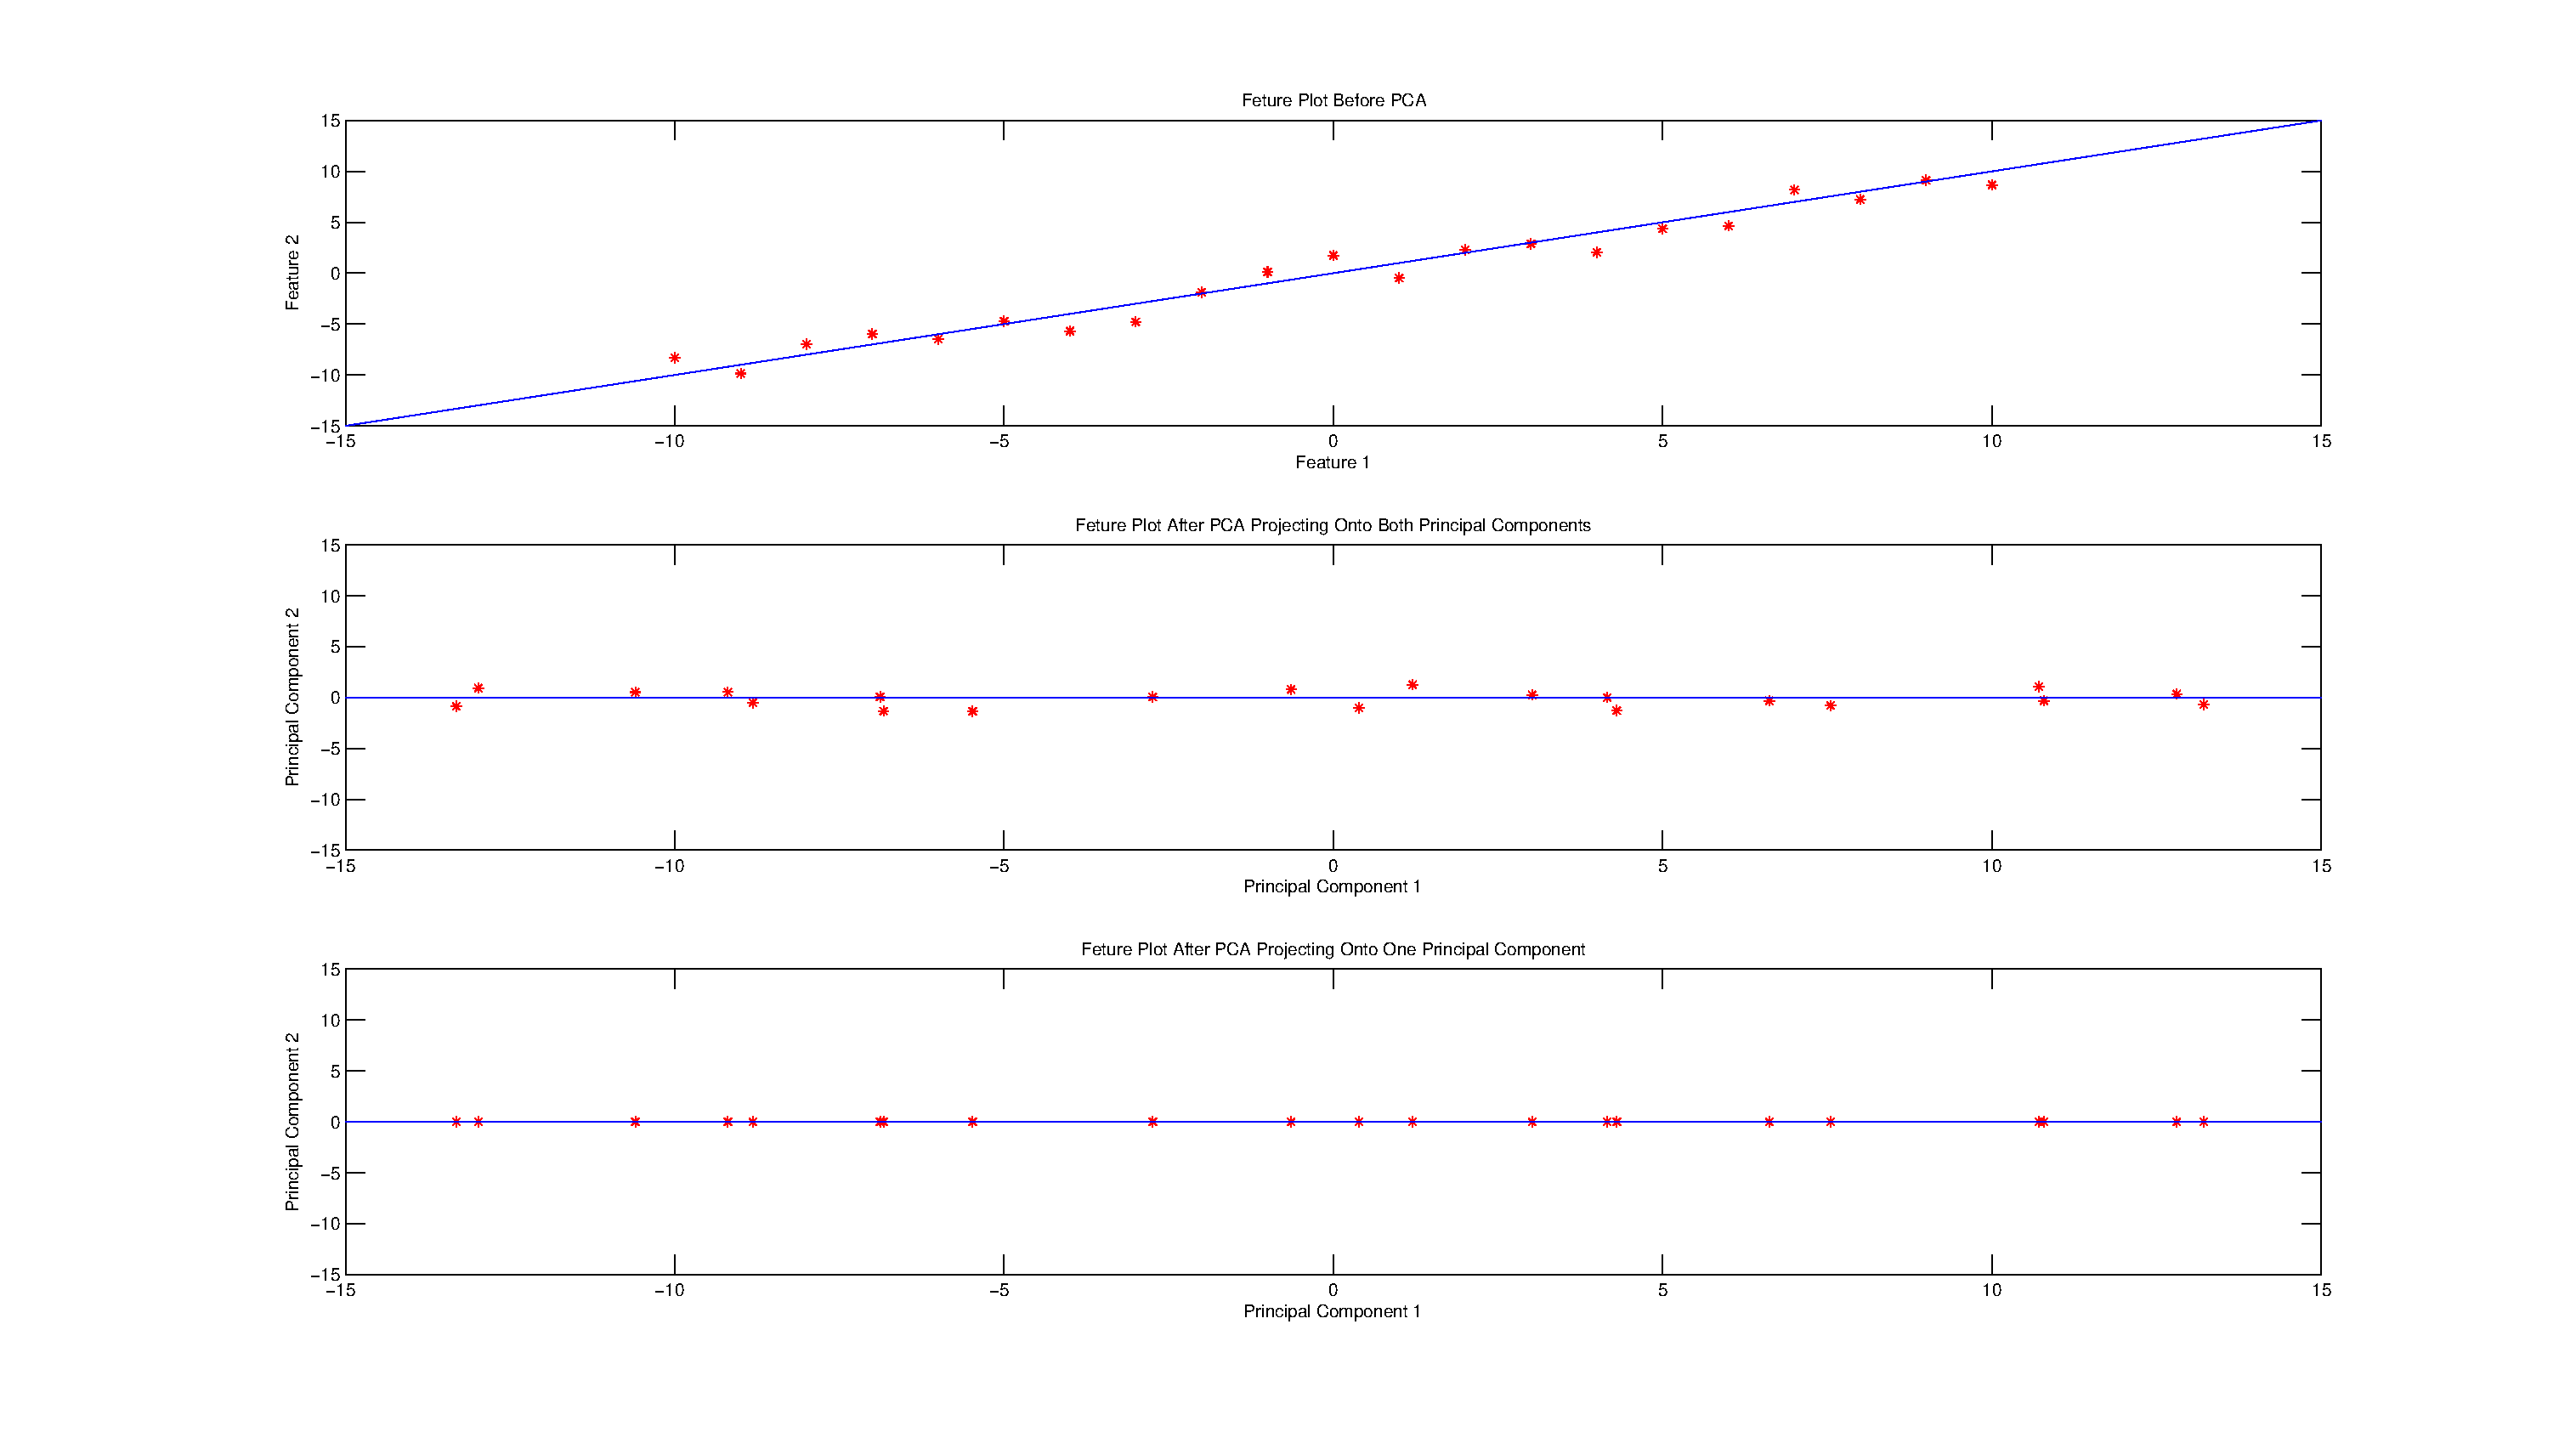
\includegraphics[height=8cm, width=10cm]{PCA_EXPLAINED.eps}
\label{pca}
\end{figure}
\end{frame}

\begin{frame}
\frametitle{Sparse PCA}
\begin{itemize}
\item Similar to PCA except the directions returned have few non-zero entries
\begin{equation}
\mathbf{v}_1 = \underset{\|\mathbf{x}\|_2^2 = 1, \|\mathbf{x}\|_0 = k}{\operatorname{argmax}}\left( \mathbf{x}^T\mathbf{A}\mathbf{x}\right)
\end{equation}
\item Makes the results easier to interpret
\item Unfortunately NP-hard to solve exactly
\end{itemize}
\end{frame}

\begin{frame}
\frametitle{Easier to interpret?}
\begin{itemize}
\item First:
\begin{equation}
\left(1.2389, 0.4532, 10.9876, \cdots, 30.3827, 19827, \cdots\right) 
\end{equation}
$\rightarrow$ a principal component with 3000 non-zero elements.
Second: 
\begin{equation}
\{1: 4.5678, 27: 2.890, 150: 9.5667, 1090: 5.4333\}
\end{equation}
$\rightarrow$ a sparse principal component with 4 non-zero elements corresponding to the keywords $\{$``o2'', ``muse'', ``playing'', ``tonight''$\}$
\end{itemize}
 
\end{frame}

\begin{frame}
\frametitle{How does this relate to Twitter data?}
\begin{itemize}
\item A Tweet can be represented as a vector in a Bag-Of-Words (BOW) space
\item Create a matrix, $\mathbf{S} \in \mathbb{Z^*}^{m \times n}$
\item Each row represents a Tweet and each column represents a word in the BOW
\item The (i, j)th element takes the value 1, if word j is in Tweet i, else it is 0
\item $\mathbf{A}=\mathbf{S}^T\mathbf{S}$
\item This gives us a Co-occurrence matrix
\item Element (i, j) is the number of times word i appears in the same Tweet as word j.
\item Taking the eigenvectors of this gives the directions that preserve the most variance
\item Given as loadings of the features/words

\end{itemize}
\end{frame}

\section{Achievements}
\begin{frame}
\frametitle{What's new in this project}
\begin{enumerate}
\item Modify input co-occurrence matrix
\item Choose SPCA algorithm for binary data
\item Streaming application to detect and track events
\end{enumerate}
\end{frame}

\begin{frame}
\frametitle{1. Modifying input matrix}
\begin{itemize}
\item Initial matrix given as	 $\mathbf{A}=\mathbf{S}^T\mathbf{S}$ but modified this to $\mathbf{A}=\mathbf{S}^T\mathbf{S} - \text{diag}(\mathbf{S}^T\mathbf{S})$ 
\item This removes link of words to themselves → increased focus on relationships between words
\item Multiple others also tried
\end{itemize}
\end{frame}

\begin{frame}
\frametitle{Example 1}
\begin{table}[H]
\center
\begin{tabular}{| r | l | r | l|}
\hline
\multicolumn{2}{|c|}{Matrix $\mathbf{A}$ }& \multicolumn{2}{|c|}{Matrix $\mathbf{A}_h$} \\
\hline
Index & Word &Index & Word \\
\hline
1 & haha & 121 & \textbf{terry}\\
7 & yeah  & 120 & \textbf{john} \\
3 & night&321 & \textbf{international} \\

5 & still & 908 & \textbf{retires}\\

12 & them& 772 & \textbf{retired}\\

6 & work& 1558 & \textbf{retirement} \\ 

2 & need &66 & \textbf{football} \\
 
9 & thanks& 144 & \textbf{england} \\

\hline
\end{tabular}
\caption{The first principal component of Twitter data during the period 23rd September 2012 to the 24th September 2012 for the unmodified and modified co-occurrence matrix. The index represents the rank of the word according to how frequent the word is found in the set of these Tweets. The bold words show words that do seem to be related according to events that have been confirmed.}
\label{pcs_jterry}
\end{table}
\end{frame}

\begin{frame}
\frametitle{Example 2}
\begin{table}
\center
\begin{tabular}{| r | l | r | l|}
\hline
\multicolumn{2}{|c|}{Matrix $\mathbf{A}$ }& \multicolumn{2}{|c|}{Matrix $\mathbf{A}_h$} \\
\hline
Index & Word &Index & Word \\
\hline
2 & need & 12 & \textbf{please} \\
1 & haha & 827 & \textbf{officers}  \\
4 & work &889 & \textbf{murders}  \\
3 & want & 240 & \textbf{following} \\
6 & them & 783 & \textbf{fallen}\\
10 & still & 756 & \textbf{recent}\\ 
7 & yeah&190 & \textbf{police}  \\ 
9 & only & 787 & \textbf{colleagues}  \\
\hline
\end{tabular}
\caption{The first principal component of Twitter data during the period 25th September 2012 to the 26th September 2012 for the unmodified and modified co-occurrence matrix. The index represents the rank of the word according to how frequent the word is found in the set of these Tweets. The bold words show words that do seem to be related according to events that have been confirmed.}
\end{table}
\end{frame}

\begin{frame}
\frametitle{2. Choosing the Sparse PCA Algorithm}
\begin{itemize}
\item Performance measure:
\begin{itemize}
\item[--] Cummulative Percentage of Explained Variance (CPEV)
\item[--] Sparsity compared with desired sparsity
\item[--] Speed of algorithm
\end{itemize}
\item TPower algorithm (speed) and Spannogram Algorithm (accuracy) best
\item TPower chosen for speed since needed in a streaming application 
\end{itemize} 
\end{frame}

\begin{frame}
\frametitle{3. Streaming Application}
\begin{itemize}
\item Have a sliding window over the Tweets and calculate the PCs for each window and check whether an event has occurred
\item Concerns include:
\begin{enumerate}[(a)]
\item How to detect events
\item How to track events already detected
\item How large the window size should be
\item How much to shift by upon each iteration 
\item How the application scales
\end{enumerate}
\end{itemize}

\end{frame}

\begin{frame}
\frametitle{(a) Detect events}
\begin{itemize}
\item Basic idea: PCs associated with events should have higher eigenvalues than PCs that aren't
\item Map to a probability using a logistic function
\end{itemize}
\begin{equation}
p(\lambda_i)= \frac{1}{\left( 1 + e^{-(w_0 + w_1\lambda_i)}\right)},
\label{logit}
\end{equation}

\begin{figure}[H]
\centering
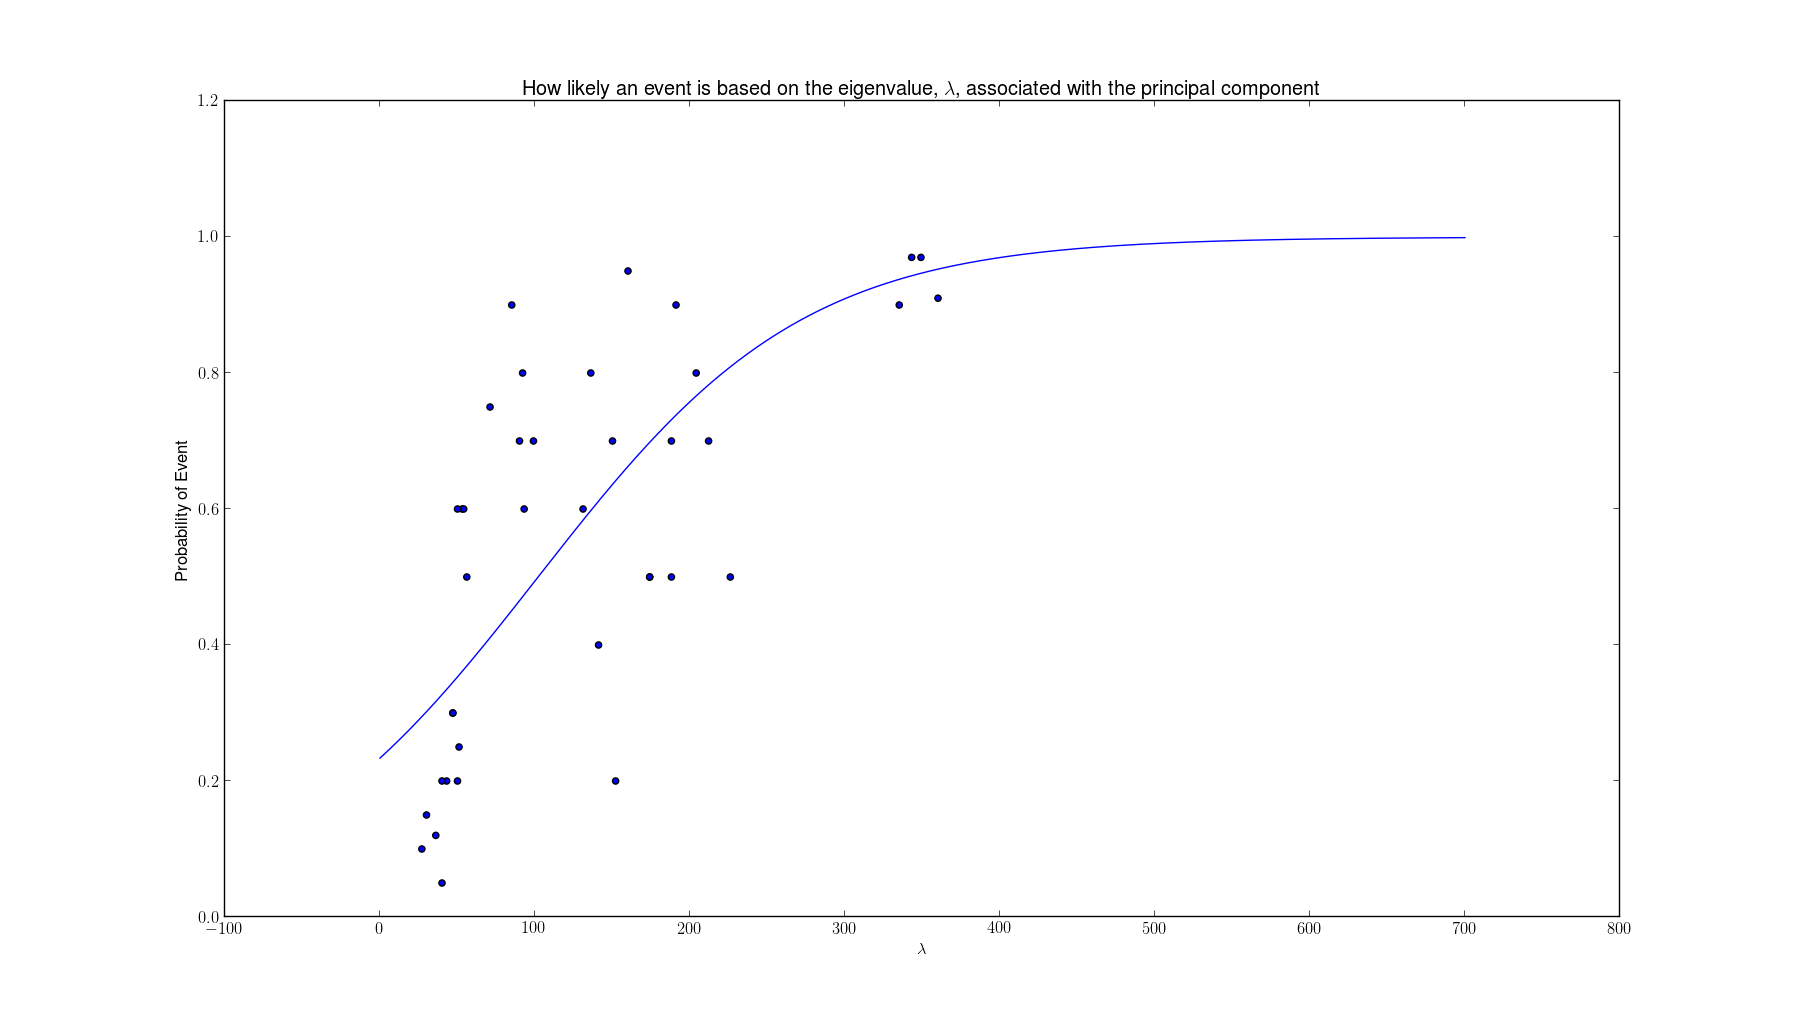
\includegraphics[scale=0.17]{Lambda_scatter.png}
\caption{An estimate of the mapping from the eigenvalue, $\lambda$, to the probability of an event. The range has been truncated to $\lambda \geq 0$ as $\lambda$ cannot take a negative value.}
\label{lambda_scatter}
\end{figure}
\end{frame}

\begin{frame}
\frametitle{(b) Track events}
\begin{itemize}
\item Tracking: to detect that an event detected is the same as the previously detected one
\item Take dot product between the two principal components and check value
\item Threshold currently = 0.85
\end{itemize}
\end{frame}

\begin{frame}[h]
\frametitle{(c) Window size - Too large}

\begin{figure}

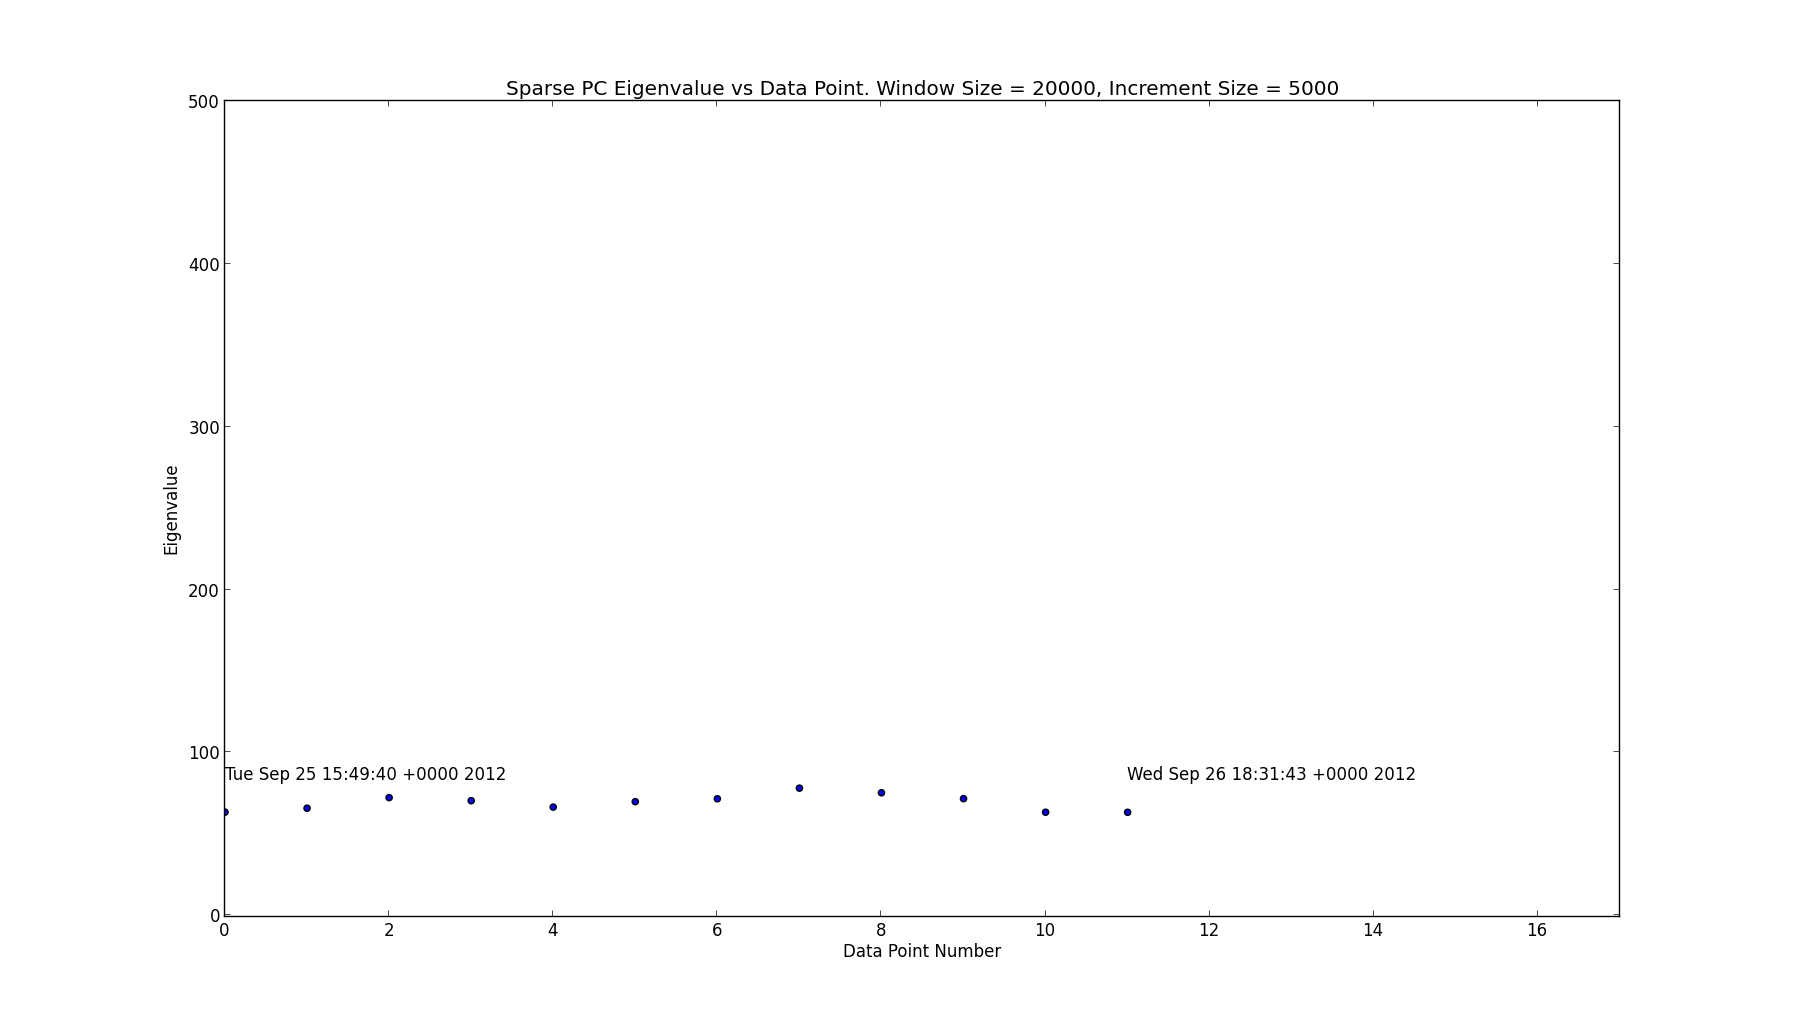
\includegraphics[scale=0.2]{Testing_Streaming_App_20000_5000.png}

\end{figure}
\end{frame}

\begin{frame}

\frametitle{(c) Window size - Too small}

\begin{figure}[h]

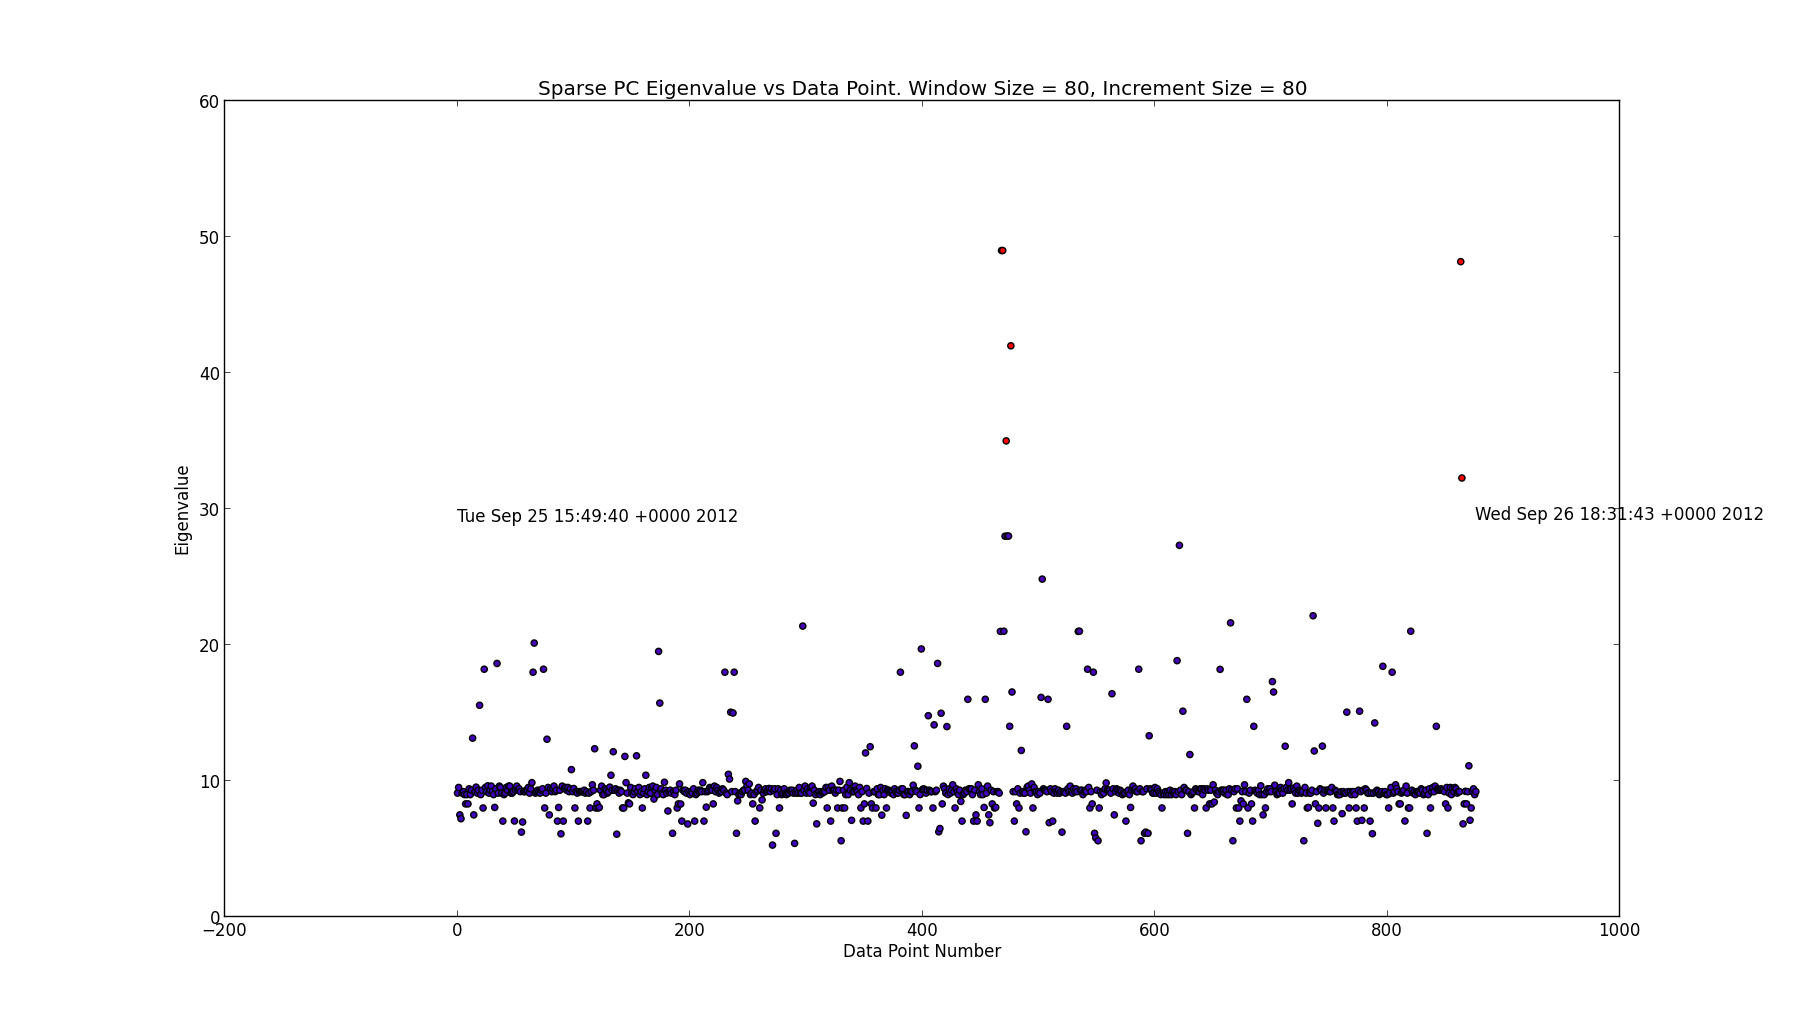
\includegraphics[scale=0.2]{Testing_Streaming_App_80_80.png}

\end{figure}

\end{frame}

\begin{frame}

\frametitle{(c) Window size - Just right}

\begin{figure}
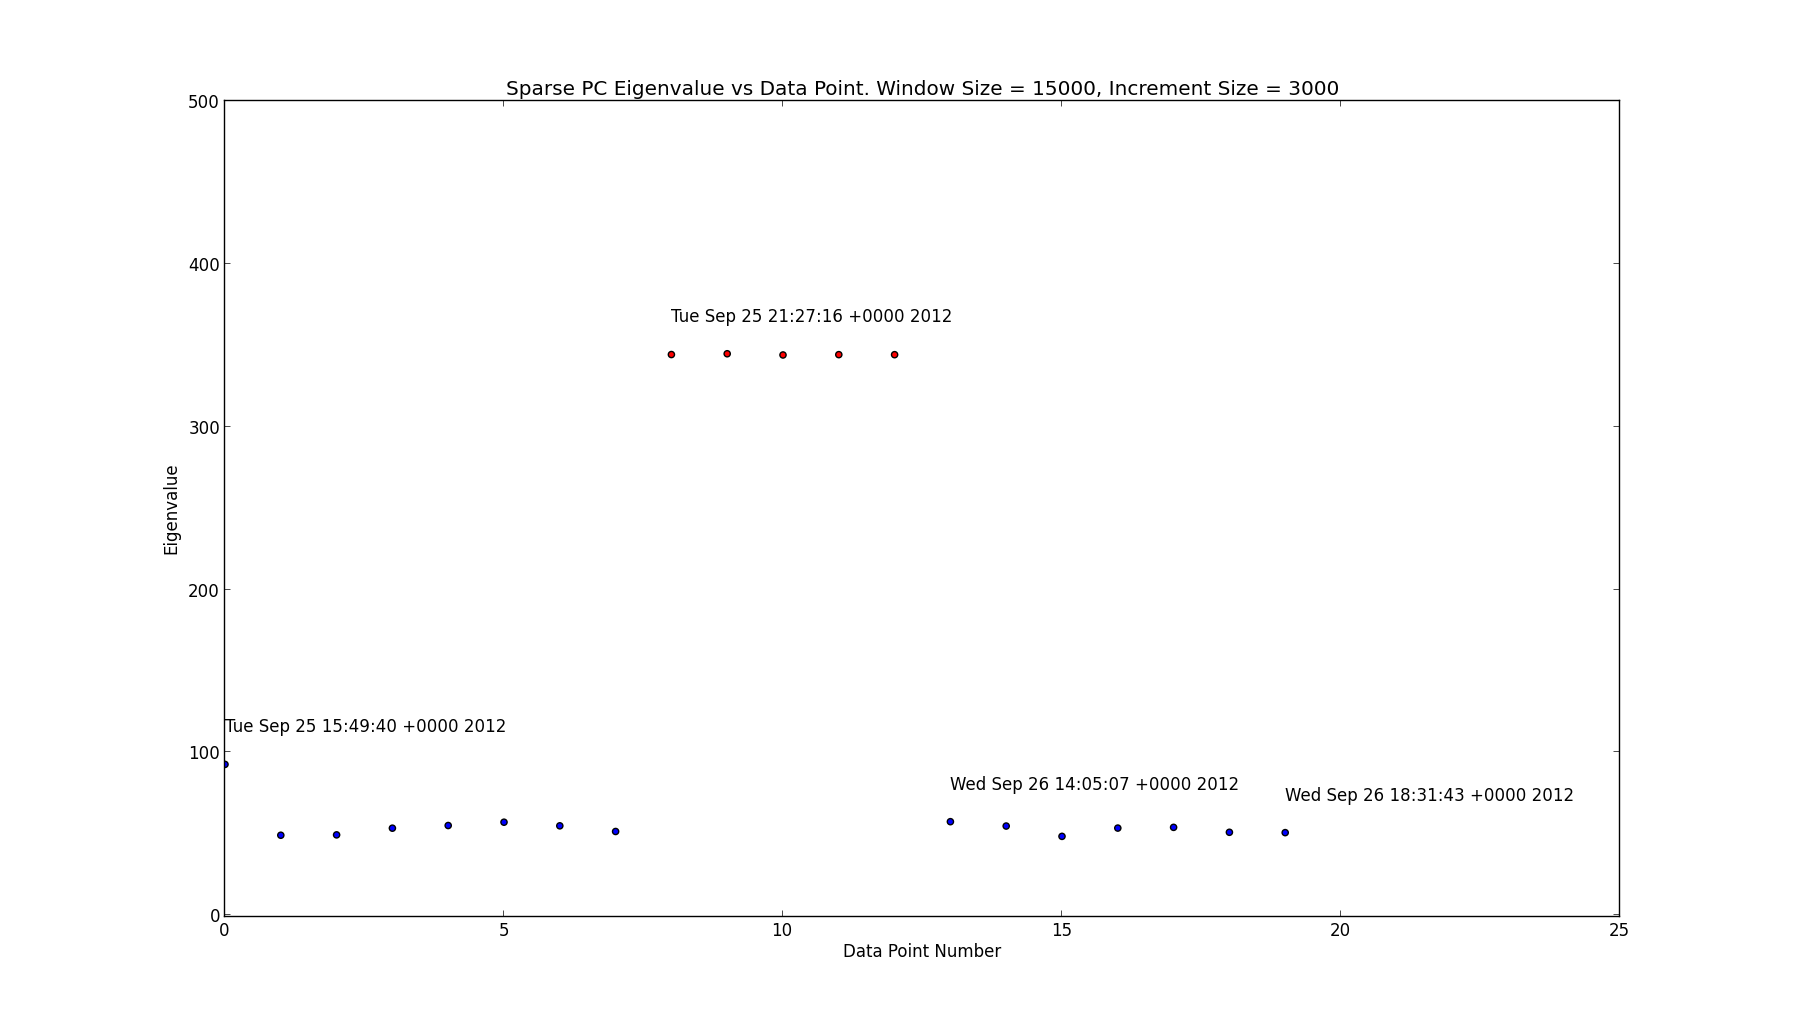
\includegraphics[scale=0.2]{Testing_Streaming_App_15000_3000.png}
\end{figure}

\end{frame}

\begin{frame}
\frametitle{Shift amount}
\begin{itemize}
\item Determined by the maximum rate of the system
\item Can decrease the shift (more overlap between window) if the rate of the Tweets is low

\end{itemize}
\end{frame}

\begin{frame}
\begin{itemize}
\item The application can work for various scales
\item Depends on geographical size considered and Twitter rate
\item Different classifier must be trained for different locations

\end{itemize}
\end{frame}
\section{Demonstration}

\section{Limitations \& Further Work}
\begin{frame}
\frametitle{Limitations}
\begin{itemize}
\item Different geographical locations need a different model to be trained for them at this point $\rightarrow$ time and effort
\item The eigenvalue alone is not a good indicator as some events have a low eigenvalue but are genuinely events (just less popular) and vice-versa
\end{itemize}
\end{frame}

\begin{frame}
\frametitle{Further Work}
\begin{itemize}
\item Clustering of features in the BOW e.g. retires, retired, retirement
\item Generalising the parameter selection process e.g. train different models for different size of locations
\item Improve event detection mechanism:
	\begin{itemize}
	\item[--] Use previous eigenvalues
	\item[--] Use the rate of Tweets
	\item[--] Use other parameters provided by the Tweet \texttt{JSON}

	\end{itemize}

\end{itemize}
\end{frame}

\section{Conclusion}
\begin{frame}
\frametitle{Conclusion}
\begin{itemize}
\item Social media provide a lot of data from which inferences can be made
\item Sparse PCA is useful for interpreting data - especially in document analysis
\item Altering the input to the Sparse PCA algorithm gives better results
\item Can create an application to find and track events in London using Sparse PCA in real-time is possible
\item Application works well for data given but must train a more general classifier
\item Room for further work

\end{itemize}
\end{frame}

\section{Summary}
\begin{frame}
\frametitle{Summary}
\begin{itemize}
\item Relevance of the project
\item Related work
\item Background information and Mathematical preliminaries
\item Achievements: Created a prototype application that can be used in a streaming fashion to detect and track events using Sparse PCA in Twitter Data.
\item Demonstration
\item Limitations
\item Further work
\item Conclusion 
\end{itemize}

\end{frame}

\section{Questions}
\begin{frame}
\frametitle{Questions?}

\end{frame}
\begin{frame}
\frametitle{References}
\bibliographystyle{ieeetr}
\bibliography{bibliography}
\end{frame}

\end{document}